\section{Experiments}
\subsection{数据集和实验设置}
我们使用的是由梅奥诊所(Mayo clinic)在2020年提供的"\emph{Low Dose CT Image and Projection Data (LDCT-and-Projection-data)}"\cite{moen2021low}公共数据集。其图像数据集总共包含25908张1mm厚度高质量CT图片来自总共150个病例。参考图像是使用FBP方法从512个投影视图生成的,我们简单地将投影数据下采样到128和64个视图,以模拟采样率分别为1/4和1/8的稀疏视图情况。150个病例分别为50个头部病例,50个胸部病例和50个腹部病例。我们将随机选取40个头部病例,40个胸部病例以及40个腹部病例作为训练集 以及 选取5个头部病例,5个胸部病例以及5个腹部病例作为验证集,再将剩下的5个头部病例,5个胸部病例以及5个腹部病例作为测试集。最终得到每个视图下训练集的总数为20800,验证集的总数为2586,测试集的总数为2522。\par
我们对比了近几年几种基于深度学习的方法的其他性能,包括FBPConvNet\cite{2016FBPConvNet},DD-Net\cite{2018DDNet},DP-ResNet\cite{2019DP-ResNet},Adaptive-Net\cite{2020ADAPTIVE},EEDeepNet\cite{2020An}。FBPConvNet是一种后处理方法,采用U-Net\cite{2015Unet}来减少FBP重构中的伪影。DD-Net结合了DenseNet\cite{2016DenseNet}和反卷积的优点,采用快捷连接将DenseNet和反卷积连接起来,提高了网络的训练速度。DP-ResNet是一种用于CT图像重建的双域网络。该算法在投影域和图像域分别对输入的测量数据进行处理,并使用FBP连接两个子网络。EEDeepNet是一种用于CT图像重建的端到端深度网络,该网络直接将稀疏的正炫图映射到CT图像上,因为原论文中并没有对其提出的网络起名,所以我们将其论文的标题“End-to-End Deep Network”简写为EEDeepNet来表示该论文所提出的网络。所有对比实验的训练参数都充分参考原论文或代码中的设置。DDPTransformer是由Adam算法\cite{2014Adam}训练的,学习率从初值$3\times10^{-4}$缓慢下降到$1 \times 10^{-6}$,mini-batch的size设为4,实验环境为Python3.8+PyTorch1.7.1在PC上(Ubuntu20.04+Intel Xeon Silver 4210R CPU+64G RAM 以及 两张 NVIDIA RTX A5000)。由于Transformer参数量和计算量巨大导致训练时间更长,我们使用PyTorch提供的DistributedDataParallel(DDP)去尽可能的缩短训练时间。所有工作的代码我们放在(github)上。另外我们通过torchRadon\cite{torch_radon}在PyTorch上实现FBP算法。\par

\textbf{Implementation details}: 在Input Projection中,我们选择尺寸为${4}\times{4}$,通道数为32的卷积核,并且为了节省空间,将stride设为4。同样在Output Projection,选择尺寸为${4}\times{4}$,通道数为32,stride为4的转置卷积。并且在Input Projection和Output Projection的卷积之后使用LeakyReLU\cite{2013Rectifier} 去稳定我们的训练。对于每个DDPTransformer Block,我们选择MSA的头数为16,并在LCL中将隐藏层的大小设为输入的四倍进行更好的学习。 我们使用了参数为0.2的Dropout\cite{2014Dropout}来防止过拟合。最后,我们将卷积层中的权重初始化为正态分布($\mu$= 0.0,$\sigma$= 0.02)。\par

\textbf{Quantitative evaluation metrics}: 通过root mean square error(RMSE),peak signal-to-noise ratio (PSNR)\cite{2008psnr},the structural similarity index metric (SSIM)\cite{2004ssim}等量化评价指标,比较了不同CT图像重建方法的性能。
RMSE的定义如下:
\begin{equation}
\begin{aligned}
\mathrm{RMSE}(X,Y) =  \frac{ \sqrt{\sum_{i}^N (X_i - Y_i)^2}}{N}   
\end{aligned}
\end{equation}
其中X表示重建结果,Y表示对应的参考图像,n is the number of pixels in a single image。
\begin{equation}
\begin{aligned}
\mathrm{PSNR}(X,Y) = 20\times\log_{10}(\frac{MAX(X,Y)}{RMSE})
\end{aligned}
\end{equation}
其中$MAX(X,Y)$表示X和Y中的最大值。
\begin{equation}
\begin{aligned}
SSIM(X,Y) = \frac{(2\mu_x\mu_y+c_1)(2\sigma_{x,y}+c_2)}{(\mu^2_x+\mu^2_y+c_1)(\sigma^2_x+\sigma^2_y+c_2)}
\end{aligned}
\end{equation}
其中$\mu$表示图像的平均值,$\sigma^2$表示图像的方差,$\sigma_{x,y}$表示两张图像的协方差。$C_1 = (0.03\times R)^2$和$C_2 = (0.01\times R)^2$是两个用来稳定具有弱分母除法的常数,其中$R$表示图像X的取值范围。用于计算ssim的图像大小为$512\times 512$。

\subsection{性能评价结果}
表一\ref{tab1}列出了在不同采样下(views = 64 and 128)的六种模型重构出测试集的CT图像的PSNR和SSIM的均值和方差,另外还给出了两种不用模型计算的参考值(FBP和bilinear+FBP)。可以看出,在不同的扫描设置下我们的网络都获得了最高的PSNR和SSIM的值以及最低的RMSE值,说明我们的网络可以重建出更高质量的CT图。和第二高的相比,PSNR在不同采样下分别高出了1.85dB(64view)和0.7dB(128view)。\par
\begin{table}[H]
	\centering
	\resizebox{\textwidth}{!}{ 
	\begin{tabular}{cccc|ccc}
		\hline
		method & PSNR & SSIM & RMSE*100 & PSNR & SSIM& RMSE*100 \\ 
		\hline
		& \multicolumn{3}{c|}{64 views} & \multicolumn{3}{c}{128 views} \\ \hline
		FBP & 20.3683$\pm$0.3074 
		& 0.3141$\pm$0.0113 
		& 1.2390$\pm$0.0831
		& 24.8409$\pm$0.2854 
		& 0.5076$\pm$0.0115
		& 0.4033$\pm$0.0261 \\
		bilinear+FBP 
		& 21.4815$\pm$0.1842
		& 0.5326$\pm$0.0182
		& 0.7301$\pm$0.0307
		& 25.0491$\pm$0.2243
		& 0.6682$\pm$0.0215 
		& 0.3195$\pm$0.0164 \\
		FBPConvNet 
		& 27.7944$\pm$0.1953 
		& 0.6584$\pm$0.0074 
		& 0.1729$\pm$0.0076
		& 34.1109$\pm$0.3703
		& 0.8635$\pm$0.0104
		& 0.0398$\pm$0.0033 \\
		DD-Net 
		& 26.8456$\pm$0.2214
		& 0.6415$\pm$0.0089 
		& 0.2132$\pm$0.0110
		& 33.0648$\pm$0.3304
		& 0.8320$\pm$0.0102
		& 0.0512$\pm$0.0041 \\			
		DP-ResNet 
		& 23.5609$\pm$0.2156
		& 0.6210$\pm$0.0194
		& 0.4469$\pm$0.0221
		& 29.8236$\pm$0.3308
		& 0.7437$\pm$0.0195
		& 0.1076$\pm$0.0085 \\
		Adaptive-Net 
		& 24.2013$\pm$0.3093 
		& 0.6462$\pm$0.0290
		& 0.3856$\pm$0.0275			
		& 31.7390$\pm$0.6146
		& 0.7853$\pm$0.0271 
		& 0.0692$\pm$0.0095 \\
		EEDeepNet 
		& 23.4033$\pm$0.2300 
		& 0.5975$\pm$0.0247
		& 0.4636$\pm$0.0246 
		& 34.2305$\pm$0.6116 
		& 0.8707$\pm$0.0148 
		& 0.0388$\pm$0.0052 \\
		DDPTransformer 
		& \textcolor{red}{29.6453}$\pm$0.9910
		& \textcolor{red}{0.7590}$\pm$0.0495
		& \textcolor{red}{0.1129}$\pm$0.0236
		& \textcolor{red}{34.8335}$\pm$1.8713
		& \textcolor{red}{0.8731}$\pm$0.0385
		& \textcolor{red}{0.0362}$\pm$0.0126 \\ 
		\hline
	\end{tabular}}
	\caption{不同方法的性能评价结果(均值$\pm$方差),最好的值用红色标出。}
	\label{tab1}
\end{table}
\subsection{视觉效果图}
图4\ref{fig4}显示了64views下不同器官(头部,胸部和腹部)的重建结果。可以看到通过FBP重建出的CT图像有很严重的条纹伪影。并且不同的模型对条纹伪影的抑制程度不同,有的甚至还会降低图像分辨率(如bilinear+FBP和AdaptiveNet)。尽管由于views过于稀疏,导致每个方法重建出的CT图像都与原图有明显差异,但DDPTransformer相比与其他方法相比仍然有最好的视觉效果。图5\ref{fig5}显示了来自128views下的重建结果。可以看到由于views的增加,每个模型重建出的图像更加清晰。但由于DDPTransformer可以获得更多的全局信息,可以看出在清晰度和图像的轮廓上效果依然是最好的,和其他相比效果更接近于原图。图6\ref{fig6}我们列出了图4和图5中选取的测试集样本的psnr,ssim和rmse值,第一行表示64view下的值,第二行表示128view下的值。图7\ref{fig7}和图8\ref{fig8}分别表示图4和图5中的roi区域(红色虚线框),我们可以看到,我们的方法重建的CT图像可以保留更多的细节。\par
\begin{figure}
	\centering
	\includegraphics[height=6cm,width=18cm]{7.eps}
	\caption{64 views 不同器官的CT重建结果图。第一行是头部,第二行是胸部,第三行是腹部}
	\label{fig4}
\end{figure}
\begin{figure}
	\centering
	\includegraphics[height=6cm,width=18cm]{8.eps}
	\caption{128 views 不同器官的CT重建结果图。第一行是头部,第二行是胸部,第三行是腹部}
	\label{fig5}
\end{figure}
\begin{figure}
	\centering
	\includegraphics[height=8cm,width=15cm]{10.eps}
	\caption{图4和图5的评价指标,第一、二行分别为64、128views下不同的评价指标。n表示头部,c表示胸部,l表示腹部。}
	\label{fig6}
\end{figure}
\begin{figure}
	\centering
	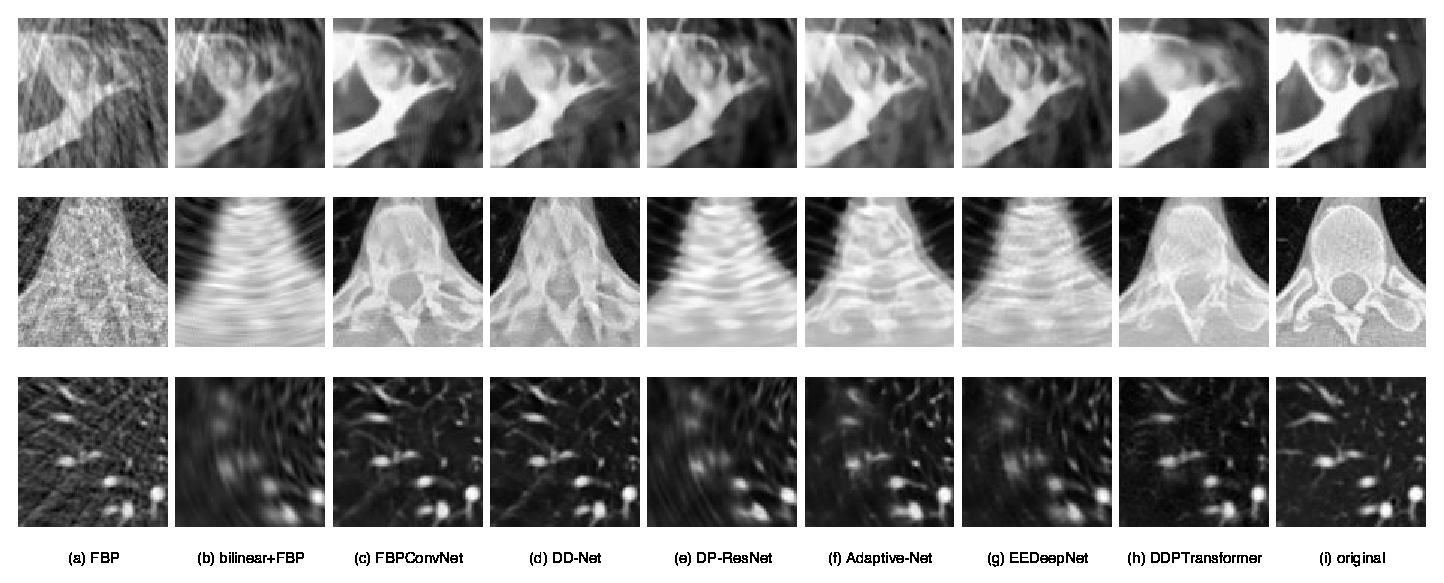
\includegraphics[height=7cm,width=18cm]{14.eps}
	\caption{图4(i)中红色框标记的缩放区域}
	\label{fig7}
\end{figure}
\begin{figure}
	\centering
	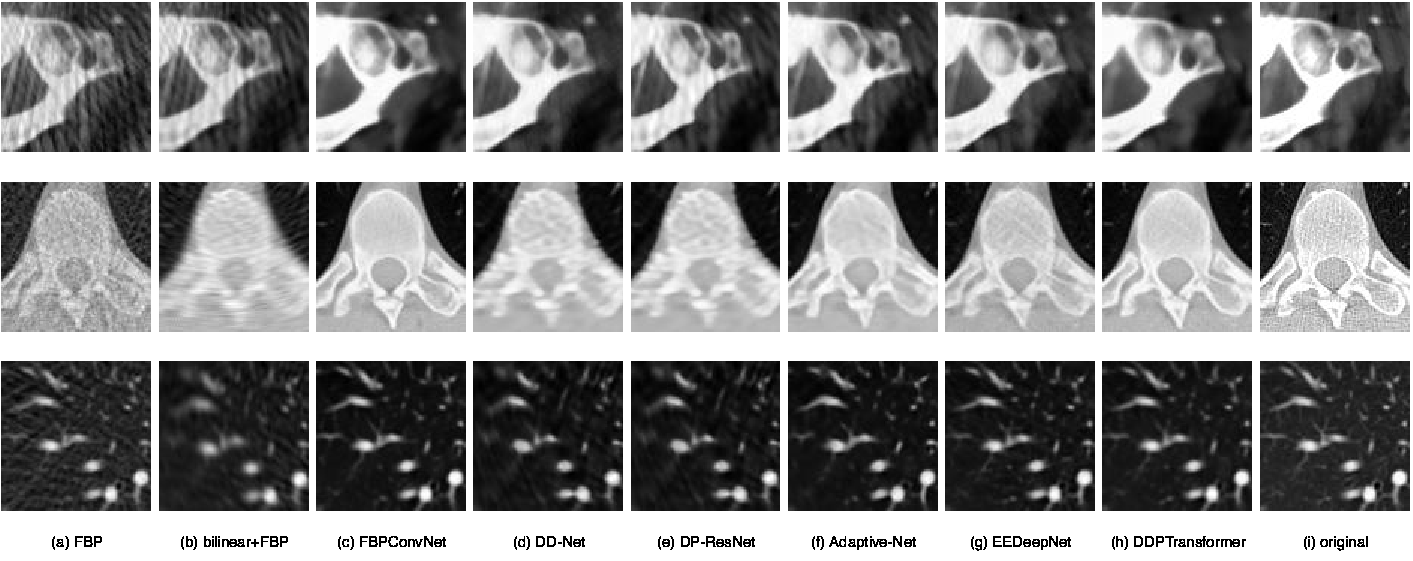
\includegraphics[height=7cm,width=18cm]{15.eps}
	\caption{图5(i)中红色框标记的缩放区域}
	\label{fig8}
\end{figure}
\subsection{Ablation Study}
在本节中,我们将评估所提出方法中不同组件的有效性。如验证Sinogram Domain SubNet(SD-Net)和Image Domain SubNet(ID-Net)的有效性、确定DDPTransformer block的个数$n$和$m$、每个DDPTransformer block只有单个Transformer(SiT)或者serial Transformer(SeT)。通过对一个参数进行改动,使其他参数保持不变,并对验证数据集的重构CT图像进行定量分析,确定各参数的最佳值。计算验证集中所有CT图像的PSNR、SSIM值和RMSE值。\par
表2\ref{tab2}列出了SD-Net和ID-Net的性能评价结果,可以看出单个子网络的性能与DDPTransformer的差距还是比较大的。图10\ref{fig10}列出了不同DDPTransformer block个数的折线图,在SD-Net中我们设置$n$为从1到7,可以看出$n$从1到5时结果越来越好,5之后效果趋于平稳,因此我们确定了$n$为5。而ID-Net中我们选择了$m$为从1到9进行实验,可以看出当$m$为7时效果最好。表3\ref{tab3}列出了与SiT和SeT进行对比的性能结果,更好的结果说明我们用并行的方式来互补Patch块边缘信息的效果是显著的。\par
\begin{table}[H]
	\centering
	\resizebox{\textwidth}{!}{ 
	\begin{tabular}{cccc|ccc}
		\hline
		method & PSNR & SSIM & RMSE*100 & PSNR & SSIM& RMSE*100 \\
		\hline  
		& \multicolumn{3}{c|}{64 views} & \multicolumn{3}{c}{128 views} \\
		\hline
		Sinogram Domain SubNet 
			& 28.9623$\pm$0.9575
			& 0.7297$\pm$0.0466
			& 0.1323$\pm$0.0273
			& 33.7763$\pm$1.5785
			& 0.8571$\pm$0.0383
			& 0.0453$\pm$0.0143 \\
		Image Domain SubNet 
			& 21.5160$\pm$0.6347
			& 0.5450$\pm$0.0615
			& 0.7241$\pm$0.1018
			& 25.1324$\pm$0.6829
			& 0.6944$\pm$0.0617
			& 0.3142$\pm$0.0478 \\
		DDPTransformer 
			& \textcolor{red}{29.6453}$\pm$0.9910
			& \textcolor{red}{0.7590}$\pm$0.0495
			& \textcolor{red}{0.1129}$\pm$0.0236
			& \textcolor{red}{34.8335}$\pm$1.8713
			& \textcolor{red}{0.8731}$\pm$0.0385
			& \textcolor{red}{0.0362}$\pm$0.0126 \\ 
			\hline
	\end{tabular}}
	\caption{子网络的性能评价结果(均值$\pm$方差),最好的值用红色标出。}
	\label{tab2}
\end{table}
\begin{figure}
	\centering
	\includegraphics[height=8cm,width=15cm]{12.eps}
	\caption{Sinogram Domain SubNet(第一行)和Image Domain SubNet(第二行)中的block个数。}
	\label{fig10}
\end{figure}
\begin{table}[H]
	\centering
	\resizebox{\textwidth}{!}{ 
		\begin{tabular}{cccc|ccc}
		\hline
		method & PSNR & SSIM & RMSE*100 & PSNR & SSIM& RMSE*100 \\  
		\hline
		& \multicolumn{3}{c|}{64 views} & \multicolumn{3}{c}{128 views} \\ \hline
		Single Transformer 
			& 27.4160$\pm$0.3170
			& 0.6693$\pm$0.0194 
			& 0.1848$\pm$0.0135
			& 30.9338$\pm$0.4125 
			& 0.7783$\pm$0.0164 
			& 0.0828$\pm$0.0077 \\
		Serial Transformer 
			& 27.8340$\pm$0.2849 
			& 0.7104$\pm$0.0170 
			& 0.1677$\pm$0.0107 
			& 32.7085$\pm$0.4841
			& 0.8350$\pm$0.0144
			& 0.0551$\pm$0.0060 \\
		DDPTransformer 
			& \textcolor{red}{29.6453}$\pm$0.9910
			& \textcolor{red}{0.7590}$\pm$0.0495
			& \textcolor{red}{0.1129}$\pm$0.0236
			& \textcolor{red}{34.8335}$\pm$1.8713
			& \textcolor{red}{0.8731}$\pm$0.0385
			& \textcolor{red}{0.0362}$\pm$0.0126 \\ 
		\hline
	\end{tabular}}
	\caption{不同Transformer的性能结果 (均值$\pm$方差),最好的值用红色标出。}
	\label{tab3}
\end{table}
\subsection{Running Time Comparisons}
在NVIDIA RTX A5000 GPU上我们对运行时间进行测试。如表4\ref{tab4}所示,尽管与卷积相比Transformer在参数量、训练时间和难度上都有巨大的优势,但在单张切片上DDPTransformer的测试时间(即不计算梯度的反向传播算法)却与其他卷积网络相差不大。在几乎相同的运行时间中,DDPTransformer实现了卓越的性能。
\begin{table}[H]
	\centering
	\begin{tabular}{cccccccc}
		\hline
		FBP & bilinear+FBP & FBPConvNet & DD-Net & DP-ResNet & Adaptive-Net & EEDeepNet & DDPTransformer\\ 
		\hline
		222 & 210 & 180 & 121 & 211 & 148 & 78 & 204 \\
		\hline
	\end{tabular}
	\caption{不同方法的运行时间(单位:ms)}
	\label{tab4}
\end{table}
